\documentclass{scrartcl}
\usepackage{includes/mypack}
\usepackage{animate}
\usepackage{courier}
\usepackage{listings}
\usepackage[T2A,T1]{fontenc}
\usepackage[utf8]{inputenc}
\usepackage[ngerman]{babel}
\usepackage[toc,page,title,titletoc]{appendix}
\definecolor{mygreen}{rgb}{0,0.6,0}
\definecolor{mygray}{rgb}{0.5,0.5,0.5}
\definecolor{mymauve}{rgb}{0.58,0,0.82}
\lstset{ %
  backgroundcolor=\color{white},   % choose the background color; you must add \usepackage{color} or \usepackage{xcolor}; should come as last argument
  basicstyle=\footnotesize\ttfamily,        % the size of the fonts that are used for the code
  breakatwhitespace=false,         % sets if automatic breaks should only happen at whitespace
  breaklines=true,                 % sets automatic line breaking
  captionpos=b,                    % sets the caption-position to bottom
  commentstyle=\color{mygreen},    % comment style
  %deletekeywords={...},            % if you want to delete keywords from the given language
  %escapeinside={\%*}{*)},          % if you want to add LaTeX within your code
  extendedchars=true,              % lets you use non-ASCII characters; for 8-bits encodings only, does not work with UTF-8
  %frame=single,	                   % adds a frame around the code
  keepspaces=true,                 % keeps spaces in text, useful for keeping indentation of code (possibly needs columns=flexible)
  keywordstyle=\color{blue},       % keyword style
  language=bash,                 % the language of the code
  %morekeywords={*,...},            % if you want to add more keywords to the set
  xleftmargin=.04\textwidth,  
  numbers=left,                    % where to put the line-numbers; possible values are (none, left, right)
  numbersep=5pt,                   % how far the line-numbers are from the code
  numberstyle=\tiny\color{mygray}, % the style that is used for the line-numbers
  rulecolor=\color{black},         % if not set, the frame-color may be changed on line-breaks within not-black text (e.g. comments (green here))
  showspaces=false,                % show spaces everywhere adding particular underscores; it overrides 'showstringspaces'
  showstringspaces=false,          % underline spaces within strings only
  showtabs=false,                  % show tabs within strings adding particular underscores
  stepnumber=1,                    % the step between two line-numbers. If it's 1, each line will be numbered
  stringstyle=\color{mymauve},     % string literal style
  tabsize=4,	                   % sets default tabsize to 2 spaces
  %title=\lstname                   % show the filename of files included with \lstinputlisting; also try caption instead of title
}


\Autoren{Attenberger, Bollenmiller, Schuster, Wilhelm}
\VersuchLang{Mobile Netze - Man-In-The-Middle} %z.B. Ein Wichtiger Versuch
\VersuchKurz{MobileNetze} %z.B. EWF
\Fach{Mobile Netze} %z.B. Physik
\Studiengruppe{IG}
\Semester{SS17}
\Betreuer{Prof. Dr. Wischhof}
\Datum{\today} %falls gewünscht auf Versuchsdatum ändern, z.B. 21. November 2012

\PDFStartpage{1} %Seite die im Reader beim Start geöffnet wird
\MyParLineSkip{0.5} %Höhe der Absätze die durch \mypar erzeugt werden: 0...1

\praeinit %Initialisierung der Styles Teil 1

%umschalter zwischen WORKMODE und FINALMODE
%im Workmode gibts kein titelblatt und kein inhaltsverzeichnis,
%sodass man sich auf die arbeit an sich konzentrieren kann,
%und das setzen schneller geht. 
%wichtig: immer mindestens dreimal setzen lassen,
%wenn auf final umgeschaltet wird, 
%damit Veweise und Inhaltsverzeichnis stimmen!!!!
\setboolean{finalmode}{true}

%Umschalter zwischen draft und normal mode
%bewirkt, dass falls eingeschaltet, alle grafiken durch rahmen
%der entsprechenden größe ersetzt und dargestellt werden.
%erhöht die performance beim setzen deutlich und verhindert ablenkung 
%beim arbeiten durch bilder.
\setboolean{draftgraphics}{false}

\begin{document}
\postinit %Initialisierung der Styles Teil 2
%%AB HIER GEHT DIE ARBEIT LOS!

\listoffigures
\section{Einleitung}
Im Rahmen der Vorlesung Mobile Netze soll zunächst ein Mobilfunknetz in Betrieb genommen werden. Des Weiteren umfasst die Aufgabenstellung die Implementierung eines Features, welches vom Team in einer Projektvision definiert wird. \\

Als Projektziel des Teams J3A soll eine Man-In-The-Middle Funktionalität in einem GSM Netz integriert werden. Man-In-The-Middle bezeichnet eine Angriffsform, bei der ein Dritter den Datenverkehr zweier Gesprächspartner mitverfolgt. Dabei bleibt er unbemerkt und ist in der Lage alle Daten, die über die Kommunikationsverbindung gesendet werden, abzugreifen. Oft täuscht er den eigentlichen Gesprächspartner vor, sodass kein Verdacht geschöpft wird.\\

Der Fokus des Projekts ähnelt stark dem Prinzip des Man-In-The-Middle Angriffs. Das Ziel ist es ein Telefongespräch abzugreifen und abzuspeichern, der zwischen zwei Teilnehmern getätigt wird. Dabei sollen die abgespeicherten Daten in eine Form gebracht werden, die das Anhören lokal auf dem Rechner ermöglicht. \\

Die Umsetzung der Aufgabenstellung umfasst die Inbetriebnahme des GSM Netzes, das aus den Komponenten BTS, BSC und MSC besteht. Über Voice over IP soll der zweite Teilnehmer erreicht werden können. Alternativ zu Voice over IP war anfänglich auch die Verbindung zum zweiten Teilnehmer ebenfalls im GSM denkbar. Die minimale Anforderung besteht in der Manipulation der BTS/BSC dahingehend, dass diese die Daten abgreift und abspeichert. Das Hinterlegen einer Rufnummer, unter der der gespeicherte Anruf angehört werden kann, wurde als optionales Feature bezüglich des Projektzieles definiert.

\newpage
\section{Architektur des Osmocom Systems}


\subsection{Was ist OsmoNITB}
Bei OsmoNITB handelt es sich um ein freies Softwarepacket aus dem Osmocom-Baseband-Projekt. Dessen Zweck ist das Aufspannen und Betreiben eines GSM/ GPRS-Netzes mittels nachgebauter Implementierungen des GSM-Protokolls. OsmoNITB bringt hierfür alle erforderlichen Bestandteile, die sich tiefer im Netz als die Basisstation (BTS) befinden. 

Die Basisstation selbst wird mit OsmoBTS realisiert. Auch sie stammt vom OsmocomBB-Projekt. Die Signale hierfür werden mittels eines Software-Radiomodems (SDR) erzeugt und versendet. Wir verwendeten hierzu den USRP N210 von Ettus Research. Dieser ermöglicht es beliebige Signale bis zu einer Frequenz der Höhe 6GHz zu generieren. Um daraus überhaupt GSM-Signale zu Empfangen oder Senden zu können ist ein Transceiver notwendig. Dieses stammt ebenfalls vom OsmocomBB-Projekt und heißt OsmoTRX. Zwischen OsmoTRX und OsmoBTS werden für deren Kommunikation UDP-Nachrichten ausgetauscht. Die Anbindung dieser wiederum an OsmoNITB erfolgt durch das A-bis-Interface, einem GSM-spezifisches, standadisiertes Protokoll für den Austausch der Gespräche und Signalisierungsdaten. Es wird ebenso mittels einer freien Implementierung von OsmocomBB, namentlich "libosmo-abis" realisiert.  


\begin{figure}[h]
    \centering
    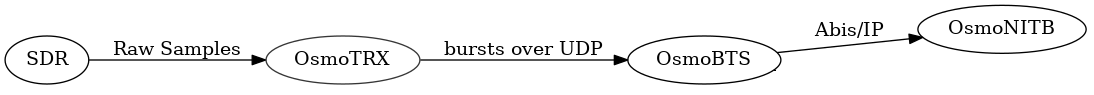
\includegraphics[width=15cm]{includes/osmotrx}
    \caption{GSM Basisstation mit OsmoTRX \& OsmoBTS}
	\label{fig:osmotrx}
\end{figure}


Der Basisstation-Controller (Base Station Controller, BSC) stellt hierbei die Gegenstelle dar und ist ebenso im OsmocomBB-Projekt enthalten. 




\begin{figure}[h]
    \centering
    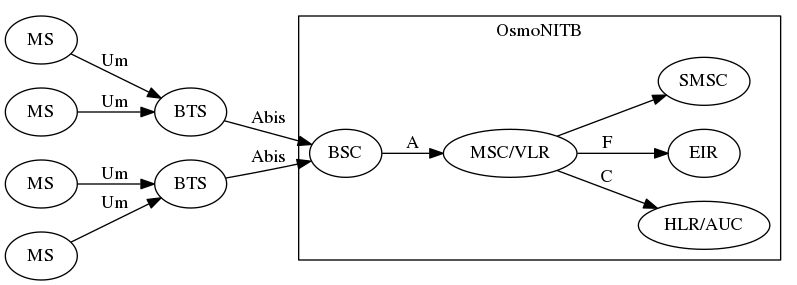
\includegraphics[width=15cm]{includes/osmonitb}
    \caption{GSM Systemarchitektur mit OsmoNITB}
	\label{fig:osmonitb}
\end{figure}



Weiterhin existieren noch folgende weitere Bestandteile, wie MSC/VLR, SMSC, EIR und HLR/AUC, die im nächsten Kapitel erklärt werden.



\subsection{Funktion der einzelnen Module}




\begin{itemize}

\item \textbf{BSC}\\
Hierbei handelt es sich wie bereits oben erwähnt um den Basisstationcontroller. Er überwacht eine Mobilfunkverbindung und regelt die Leistung nach. Zudem lösst er einen Zellenwechsel, dem sogenannten Handover aus. OsmoNITB nutzt hierzu die freie Implementierung OpenBSC.  

 
\item \textbf{MSC/VLR}\\
Die Mobile-service switching center stellt im GSM/GPRS-Netz die Vermittlungsstelle dar. Sie übernimmt die Anrufverwaltung, die Verwaltung der Authentifizierung und innerhalb eines kommerziellen Netzes auch die Gebührenerfassung. Das Visitor Location Register (VLR) würde zudem, die jeweilige Basisstation unter der ein Endgerät eingebucht ist oder zuletzt war, verwalten. Sie kennt damit den Ort des Mobilfunknutzers. Unser Projekt wird jedoch nur mit einer Basisstation durchgeführt, weshalb kein Handover nötig ist. Damit verbleibt das Mobiltelefon nur in einer Location. 


\item \textbf{SMSC}\\
Der SMSC ist ein Server für SMS-Dienste. Er kümmert sich um die Verarbeitung von Textmitteilungen. Hierunter fällt beispielsweise die Speicherung, Weiterleitung von SMS. Sie wird im weiteren Projektverlauf nicht benötigt.


\item \textbf{EIR}\\
Dies ist ein optionales Modul und wird nicht zwingend für den Betrieb eines GSM-Netzes benötig. Dabei handelt es sich um ein Equipment Identity Register (EIR). Hier werden die weltweit eindeutigen Seriennummern der Mobilgeräte (IMEI, International Mobile Equipment Identity) gespeichert. Ziel dieser Datenbank ist ein Sperren verlorener oder gestohlener Endgeräte zu ermöglichen. Auch sie wird in diesen Projekt nicht benötigt. Zudem verwenden auch im kommerziellen Betrieb nur wenige Mobilfunkbetreiber dieses, da die IMEIs oftmals verändert werden können und die Datenbank damit wirkungslos ist.  


\item \textbf{HLR/AUC}\\
HLR steht für Home Location Register und bildet die Datenbank in der die Nummer eine Mobiltelefons zu dessen eindeutigen Identifiers, der IMSI (International Mobile Subscriber Identity), hinterlegt ist. Zudem wird hier die TMSI aufgelöst. Eine temporäre IMSI, die den Nutzer eines Mobilgeräts durch Zuweisen einer veränderlichen Identifiers, besser vor Tracking schützen soll. Das Authentification Center (AUC) ist die Authentifizierungszentrale und damit der Ort, an dem der Authentifizierungsschlüssel Ki abgelegt ist. Hier wird die Authentifizierung der SIM-Karte gegenüber dem Mobilfunknetz durchgeführt. 


\end{itemize}


OsmoNITB implementiert damit das Network Switching Subsystem (NSS), aber mit dem BSC auch Teile des Base Station Subsystems (BSS). Das NSS ist hierbei der Teil der inneren Infrastruktur des Neztes, welches sich mit der Verwaltung von Mobilgeräten und Gesprächen beschäftigt. Das BSS hingegen kümmert sich im wesentlichen nur um die Verwaltung und Belegung der Funkschnittstelle.


\subsection{Funktionsweise von OsmoNITB}

In der Standardeinstellung von OsmoNITB werden Steuerungssignale von der BTS an diese weitergereicht, während die Gesprächsdaten mit Hilfe des verbindungslosen Protokoll UDP direkt an die Ziel-BTS gerichtet werden. Dazu sendet OsmoNITB in Form einer A-bis-Meldung einen Lauschbefehl an die Ziel-BTS. Eine Schicht höher wird dieses als Multimedia Protokoll RTP interpretiert. In unseren Projekt wurde die Einstellung „RTP proxy mode“ verwendet. Dies bewirkt, dass die RTP-Daten zuerst von OsmoNITB registriert werden und von dieser ausgehend nochmals an die Ziel-BTS versendet werden. Dies ist notwendig, da wir nur eine BTS betreiben, die zugleich Start-BTS und Ziel-BTS ist. Damit wird erreicht, dass dennoch ein RTP-Datenstrom detektierbar ist. Nachfolgendes Bild zeigt den prinzipiellen Aufbau eines derartigen Aufbaus:



\begin{figure}[h]
    \centering
    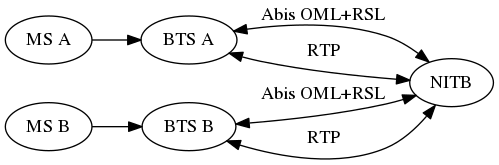
\includegraphics[width=8cm]{includes/osmonitb_rtp_proxy}
    \caption{OsmoNITB mit RTP proxy mode}
	\label{fig:osmonitb2}
\end{figure}


Weiterhin läuft auf unseren System die Telefonanlage Asterisk. Sie ist mittels Osmocom-Sip-Connector an OsmoNITB angeschlossen. Dieser generiert aus dem MNCC-Datenstrom, dem klassischen Anrufsteuerungsprotokoll von ISDN, aus OsmoNITB einen SIP-Datenstrom (Session Initiation Protocol). Mit Hilfe dieses Sitzungsprotokolls kann ein Gespräch für die Man-in-the-middle-Attacke abgefangen werden. Insgesamt ergibt sich somit für unser System folgender Aufbau:



\begin{figure}[h]
    \centering
    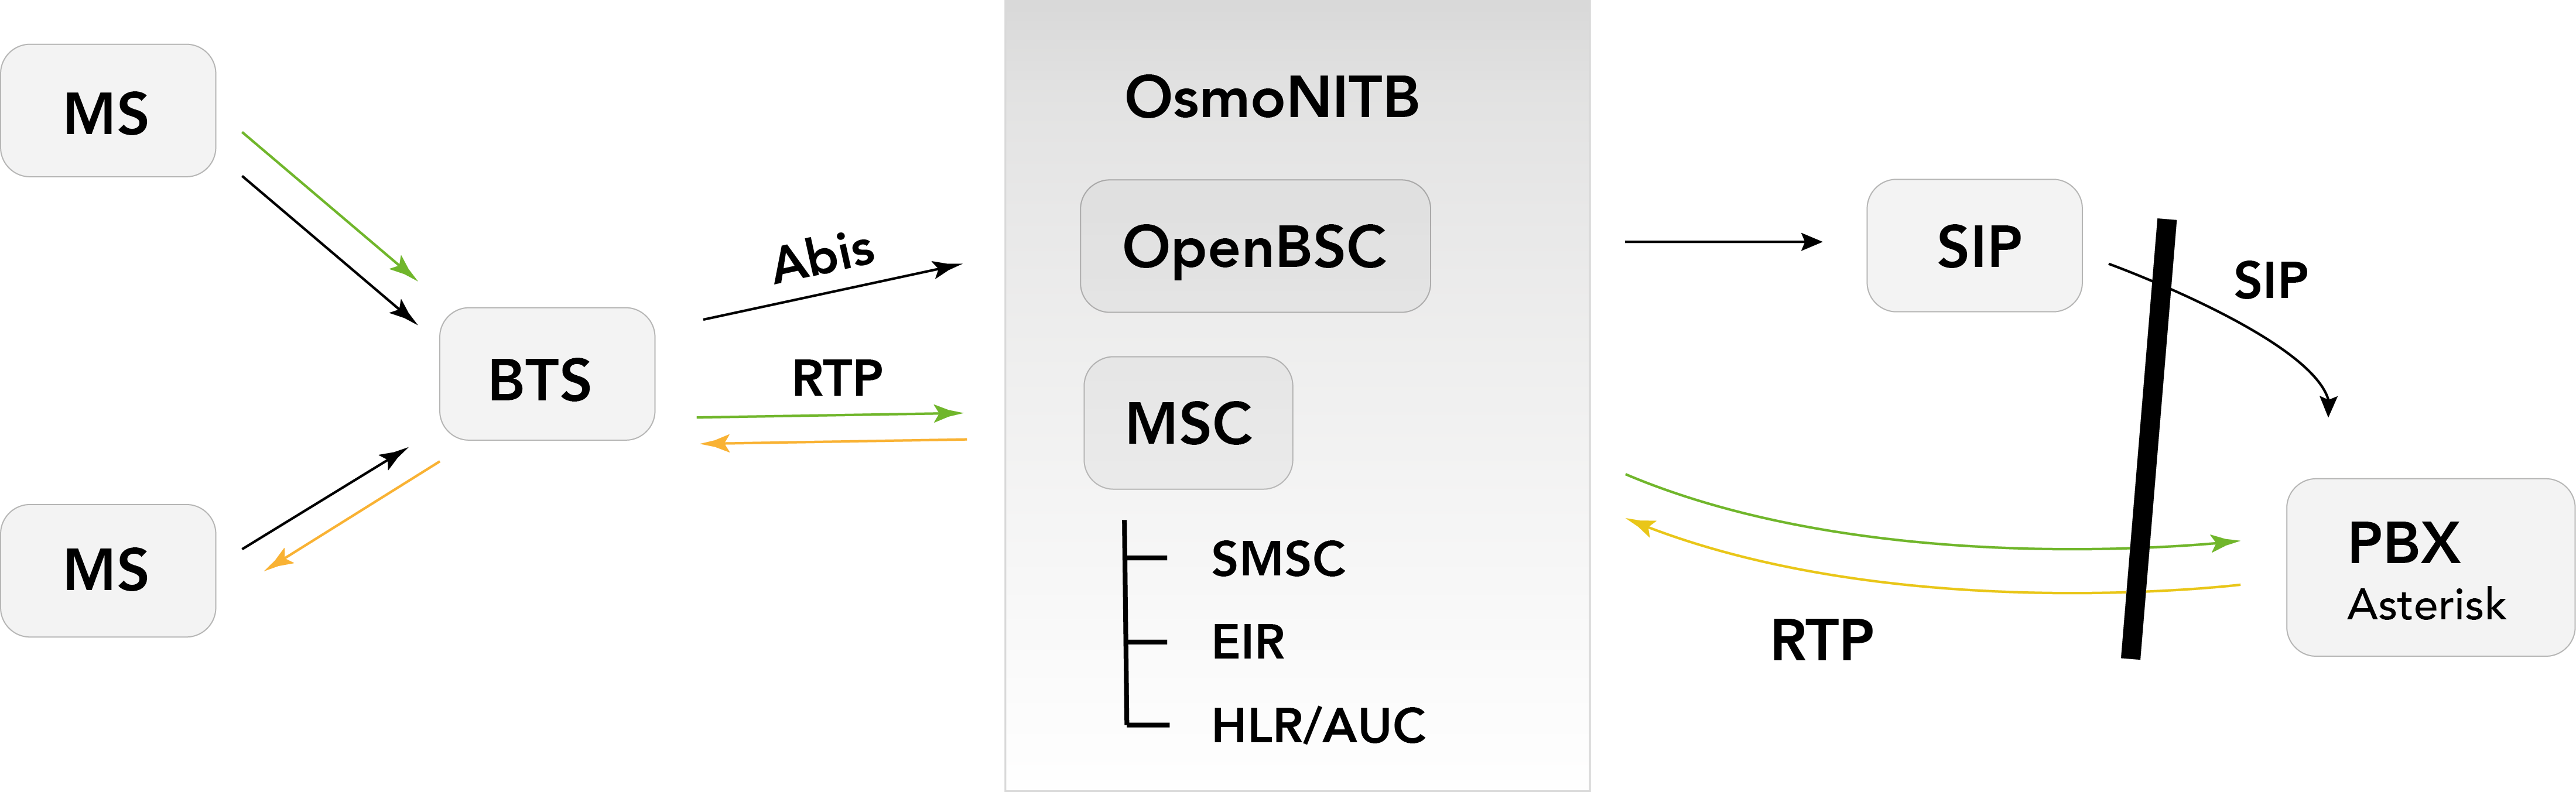
\includegraphics[width=14cm]{includes/aufbau_osmonitb}
    \caption{Unser Systemaufbau}
	\label{fig:osmonitb3}
\end{figure}


Der Datenabgriff erfolgt in unserem Fall an der Stelle des schwarzen Balkens (s. Bild oben). Wird ein Gespräch aufgebaut, so signalisiert SIP dieses und der RTP-Stream kann abgefangen werden.

\newpage
\section{Architektur des OpenBTS Systems}
OpenBTS (Open Base Transceiver Station) ist eine in C++ geschriebene, frei zugängliche Software-Suite des Unternehmens Range Networks. Zusammen mit einem Software Defined Radio (SDR) ist es möglich eine Basisstation für ein Mobilfunknetz mit GSM-Standard in Betrieb zu nehmen.
Das Projekt nahm sich unter anderem zum Ziel die Kosten zur Inbetriebnahme eines GSM-Mobilfunknetzes so gering wie möglich zu halten, um in Gebieten eingesetzt werden zu können, in denen der Aufbau eines Mobilfunknetzes mit herkömmlichen GSM-Basisstationen nicht lukrativ genug ist.\\
Eine OpenBTS-Installation besteht dabei aus mehreren Softwarepaketen, welche die verschiedenen Funktionen eines Mobilfunknetzes implementieren und die unter der AGPLv3 Lizenz von Range Networks zur Verfügung gestellt werden. Diese Softwarepakete sind zuständig für die verschiedenen Bestandteile eines Mobilfunknetzes wie Schnittstellen, SMS-Versand, Teilnehmerauthentifizierung und Anrufvermittlung im eigenen Netz sowie, je nach Anbindung, zu VoIP- und Festnetzteilnehmern.


\subsection{Aufbau und Zusammenspiel}
\subsubsection{Bestandteile}

Das vollständige OpenBTS-System beinhaltet zum Zeitpunkt des Projekts die folgenden Software-Komponenten:

\begin{itemize}
\item \textbf{OpenBTS}\\
Die eigentliche OpenBTS-Anwendung, die den Großteil des GSM-Stacks oberhalb des Radiomodems realisiert.

\item \textbf{Transceiver}\\
Ein Software-Radiomodem sowie Hardware-Kontrollsystem, welches für die Anbindung eines Software Defined Radio (SDR) zuständig ist. In unserem Fall wurde das Universal Software Radio Peripheral (USRP) N210 SDR  der Firma Ettus Research (siehe Abbildung \ref{fig:n210}) über das Netzwerk mit allen genutzten Computern verbunden.
\begin{figure}[htbp]
    \centering
    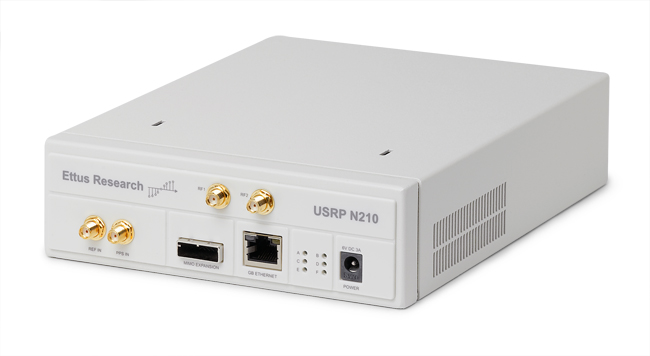
\includegraphics[width=0.90\textwidth]{includes/ettus_n210}
    \caption{USRP N210 Software Defined Radio}
	\label{fig:n210}
\end{figure}

\newpage
\item \textbf{Asterisk}\\
Um eine Gesprächsvermittlung im Mobilfunknetz realisieren zu können, wird ein Private Branch Exchange (PBX) oder SIP Softswitch wie Asterisk benötigt, welcher somit die Hauptfunktionen eines klassischen Mobile Switching Center (MSC) übernimmt. Asterisk bietet die Möglichkeit sowohl innerhalb des eigenen Mobilfunknetzes, als auch ins Festnetz und zu VoIP-Services, Gespräche aufzubauen und unterstützt weitere Features wie Sprachdienste, Mailbox-Services oder Telefonkonferenzen.

\item \textbf{SIPAuthServe}\\
SIPAuthserve verwaltet eine Subscriber Registry Datenbank, die die Teilnehmer-Informationen der im Netz registrierten Endgeräte enthält - unter anderem IMSI und Rufnummer. Diese Datenbank dient als Ersatz für das Home Location Register (HLR) eines klassischen GSM-Netzes sowie die SIP Registry von Asterisk.

\item \textbf{SMQueue}\\
SMQueue ist ein RFC-3428 Store-and-Forward Message Service für die Übertragung und Speicherung von SMS-Nachrichten. Es verfügt über einen Shortcode-Handler, welcher es ermöglicht den Inhalt von Textnachrichten als Eingabeargumente zu nutzen. So beinhaltet SMQueue standardmäßig einen Registrierungsprozess, der Benutzern dabei hilft eine gewünschte Rufnummer zu registrieren.
\end{itemize}

Die Beziehungen und Verbindungsprotokolle aller Komponenten eines OpenBTS-Systems werden in Abbildung\ref{fig:openbts} dargestellt. Dabei repräsentieren eckige Boxen Hardware-Komponenten, abgerundete Boxen Software-Komponenten.
\begin{figure}[htbp]
	\centering
		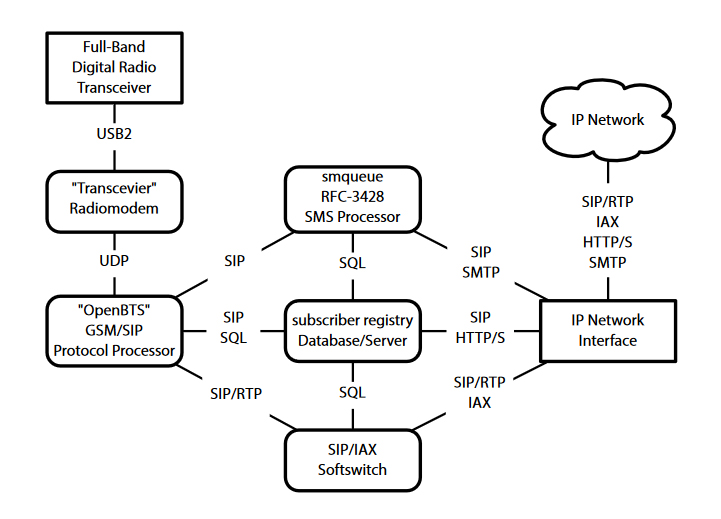
\includegraphics[width=1.00\textwidth]{includes/openbts}
	\caption{OpenBTS Systembestandteile}
	\label{fig:openbts}
\end{figure}

\newpage

\subsubsection{Datenbanken}
Da in OpenBTS viele unterschiedliche Software-Komponenten miteinander interagieren, werden auch mehrere Datenbanken für Einstellungen oder die Kommunikation zwischen verschiedenen Komponenten benötigt. Die folgenden Datenbanken kommen dabei zum Einsatz:

\begin{table}[h]
	\centering
		\begin{tabular}{ll}
			\textbf{OpenBTS.db} & Enthält alle Konfigurationseinstellungen des OpenBTS-Hauptprogramms.\\
			& Die Einstellungen der für uns lizenzierten Frequenz, sowie Netzwerk-\\
			& parameter wie MCC, MNC oder Name können hier gesetzt werden.\\
			\textbf{TMSITable.db} & Enthält die TMSI-IMSI Beziehungen der registrierten Endgeräte und wird\\
			& vom OpenBTS-Hauptprogramm genutzt. Der Pfad wird als Parameter in\\
			& der OpenBTS.db-Datenbank gesetzt.\\
			\textbf{ChannelTable.db} & Enthält den Channel Status aller aktiven Channel und wird vom OpenBTS-\\
			& Hauptprogramm genutzt. Der Pfad wird als Parameter in der OpenBTS.db-\\
			& Datenbank gesetzt.\\
			\textbf{sipauthserve.db} & Enthält alle Konfigurationseinstellungen von SIPAuthServe, unter anderem\\
			& den Dateipfad zur Subscriber Registry (sqlite3.db).\\
			\textbf{smqueue.db} & Enthält alle Konfigurationseinstellungen von SMQueue, unter anderem\\
			& den Dateipfad zur Subscriber Registry (sqlite3.db).\\
			\textbf{sqlite3.db} & Subscriber Registry, auf die von SIPAuthServe und SMQueue zugegriffen\\
			& wird. Wenn Asterisk mit Real-Time Funktionen konfiguriert wird, greift\\
			& auch Asterisk via ODBC auf die sqlite3-Datenbank zu.\\
		\end{tabular}
\end{table}

Der Kommunikationsfluss der OpenBTS-Komponenten über die Datenbanken ist in Abbildung \ref{fig:openbts_system_diagram} dargestellt. \textbf{Schwarze} Pfeile bezeichnen SIP-Verbindungen, \textcolor{red}{\textbf{rote}} Pfeile stellen Datenbankzugriffe dar und der \textcolor{blue}{\textbf{blaue}} Pfeil eine ODBC-Verbindung, die nicht standardmäßig in OpenBTS integriert ist und die zusätzlich für Asterisk Real-Time konfiguriert werden muss.
\begin{figure}[htbp]
	\centering
		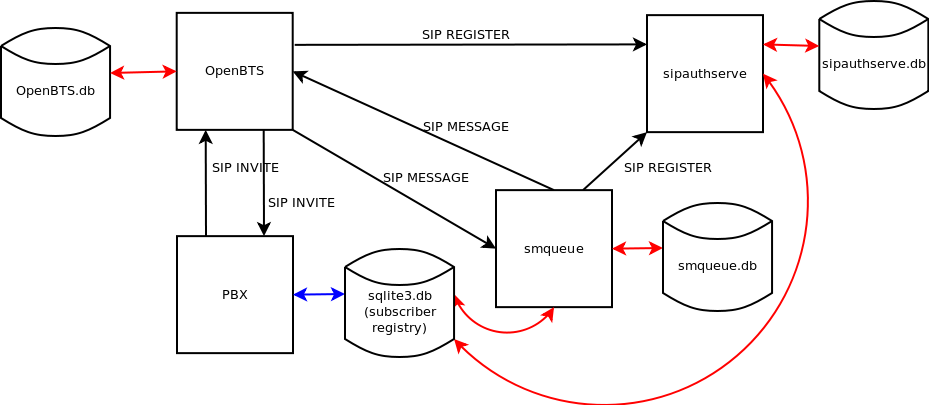
\includegraphics[width=1.00\textwidth]{includes/openbts_system_diagram}
	\caption{OpenBTS System Diagramm}
	\label{fig:openbts_system_diagram}
\end{figure}




\newpage
\subsection{}
\newpage

\section{Inbetriebnahme eines Osmocom Systems}
Für Inbetriebnahme des GSM Netzes waren einige Vorinstallationen sowie das Einrichten von Ubuntu 16.04.3 nötig. Im Folgenden wird das Vorgehen zur Einrichtung des Systems sowie die Inbetriebnahme des GSM Netzes beschrieben.

\subsection{Vorinstallationen}

\subsubsection{Ubuntu 16.04.3}
Zunächst wurde das Betriebssystem Ubuntu 16.04.3 auf einem Labor-Rechner installiert und eingerichtet.

\subsubsection{Git}
Da die Open-Source Projekte von OsmocomBB auf Git-Repositories liegen, wurde zunächst Git eingerichtet. Zur Versionskontrolle und Verwaltung des Codes wurde außerdem ein Team-eigenes Git Repository angelegt.

\begin{lstlisting}
sudo apt-get install git
\end{lstlisting}

\subsubsection{Softwarevoraussetzungen}
Osmocom empfiehlt zunächst die Einrichtung von einigen Bibliotheken und sonstigen, nötigen Abhängigkeiten als Voraussetzung für die Inbetriebnahme der GSM Komponenten. Diese wurden mittels Paketmanagers wie folgt installiert.

\begin{lstlisting}
sudo apt-get install libpcsclite-dev libtalloc-dev libortp-dev libsctp-dev 
libmnl-dev libdbi-dev libdbd-sqlite3 libsqlite3-dev sqlite3 libc-ares-dev 
libdbi0-dev libdbd-sqlite3 build-essentials libtool autoconf automake pkg-config 
libsqlite3-tcl sqlite-autoconf sqlite-autoconfg
\end{lstlisting}

Die die Fehler bezüglich Bumpversion nicht behoben werden konnten, wurden sie ignoriert. Dies zog keinerlei Konsequenzen hinsichtlich der Inbetriebnahme der GSM Komponenten nach sich.

Zusätzlich bedarf es der separaten Installation der Software Bibliotheken libosmo-abis, libosmocore und libosmo-netif. Diese wurden von den entsprechenden Git Repositories heruntergeladen und nach analogem Vorgehen installiert.

\begin{lstlisting}
git clone git://git.osmocom.org/<lib-source>
cd <lib-source>
autoreconf -fi
./configure
make
make install
sudo ldconfig
\end{lstlisting}

Trotz der sorgfältigen Installation einiger Softwarevoraussetzungen traten zusätzliche Abhängigkeiten bei der Installation einzelner GSM Komponenten auf, welche in \ref{GSM_Komp_Osmocom} beschrieben sind.

\subsubsection{Aktivierung der Verbindung zum USRP2}
Vor Installation des Treibers sollte zunächst die Netzwerkschnittstelle wie folgt aktiviert werden. Die default IP Adresse des Ettus USRP2 ist 192.168.10.2. 

\begin{lstlisting}
sudo ifconfig enp0s25 192.168.10.3
ping 192.168.10.2
\end{lstlisting}

\subsection{Installation einzelner GSM Komponenten}\label{GSM_Komp_Osmocom}
OsmocomBB hält detaillierte Beschreibungen zur Installation der GSM Komponenten bereit, welche zur Inbetriebnahme des in Rahmen dieser Arbeit verwendeten GSM Netzes herangezogen wurden. Im Folgenden wird die Installation und Einrichtung der GSM Komponenten genauer erläutert. 

\subsubsection{OsmoTRX}
Zur Kommunikation mit der Basisstation ist der osmoTRX Transceiver nötig. Osmocom bietet diesen - meist wie die anderen Komponenten - im Git Repository an. Die Installation des Transceiver erforderte die Bibliotheken \textit{$libusb-1.0-0-dev$, $uhd-host$, $libboost-dev$} und \textit{$libuhd-dev$}. Diese bieten die Suchfunktion \textit{uhd\_find\_devices}. Dadurch lässt sich testen, ob die Basisstation gefunden wird. Mittels \textit{osmo-trx} lässt sich der Transceiver nach der Installation starten.

\begin{lstlisting}
git clone git://git.osmocom.org/osmo-trx
cd osmo-trx/
autoreconf -i
./configure
sudo make -j8
sudo make install
osmo-trx	
\end{lstlisting}

\begin{figure}[h] %t=top b=bottom h=here p =eigene page
\centering
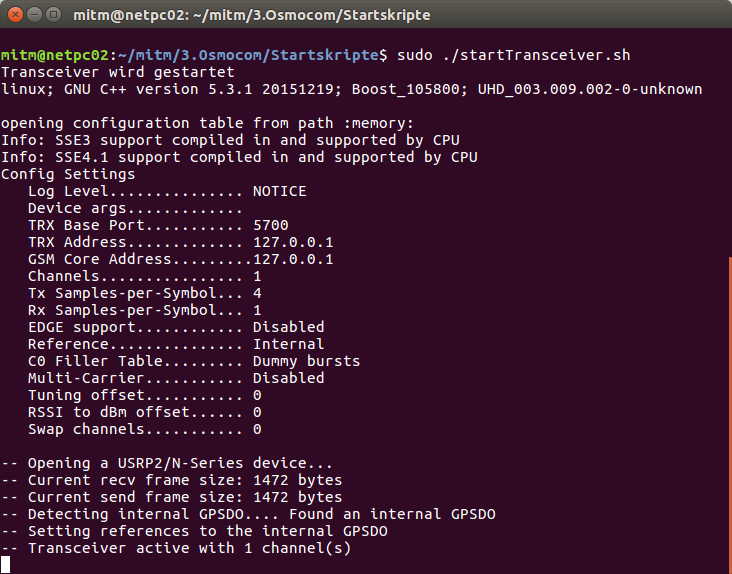
\includegraphics[width=15cm]{includes/Start_Transceiver}
\caption{Ansicht der Konsole nach dem Start des Transceivers}
\label{fig:Transceiver}
\end{figure}

Zur Behebung der Warnung, die in Abbildung \ref{fig:UHDWarnung} zu sehen ist, wurde die Priorität in der Datei /etc/security/limits.conf gesetzt.

\begin{lstlisting}
@usrp   -  rtprio  50
\end{lstlisting}

\begin{figure}[h] %t=top b=bottom h=here p =eigene page
\centering
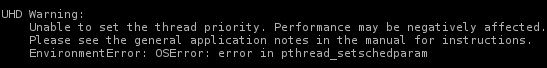
\includegraphics[width=15cm]{includes/uhd_usrp_warnung}
\caption{Fehlermeldung bezüglich der Thread Priorität in osmoTRX}
\label{fig:UHDWarnung}
\end{figure}

\subsubsection{OsmoBTS}
Die Installation von OsmoBTS erfolgte analog zur Einrichtung der anderen Osmocom Komponenten.

\begin{lstlisting}
git clone git://git.osmocom.org/osmo-bts.git
autoreconf -fi
cd osmo-bts
./configure --enable-trx
sudo make -j8
sudo make install
\end{lstlisting}

Zur Konfiguration wurden zunächst die Pfade der folgenden Variablen angepasst.

\begin{lstlisting}
PATH="/usr/local/sbin:/usr/local/bin:/usr/sbin:/usr/bin:/sbin:/bin:/usr/games:/usr/local/games"
PKG_CONFIG_PATH="/home/netpc06/libosmo-abis/"
LIBOSMOTRAU_CFLAGS="/home/netpc06/libosmo-abis/"
LIBOSMOTRAU_LIBS="/home/netpc06/libosmo-abis/"
\end{lstlisting}

Weiterhin erforderte die Konfiguration von OsmoBTS Änderungen an der Datei osmo-bts.cfg (siehe Anhang \ref{Osmo-bts.cfg}). Es wurde die Option \textit{band} auf PCS1900 gesetzt, welche dem lizenzierten Frequenzband entspricht. Des Weiteren wurde    die Signalstärke durch Angabe des \textit{osmotrx rx-gain} auf 1 gesetzt. Eine letzte Änderung wurde an der lokalen und remote IP vorgenommen, welche auf 127.0.0.1 gesetzt wurde. \\

Die Konfigurationsdatei wurde unter dem Pfad \textit{/home/netpc06/osmo-bts/src/osmo-bts-trx} abgelegt. 

\subsubsection{OsmoNitb unter OpenBSC}
Weiterhin wurde OpenBSC installiert. Dazu wurde die Bibliothek libssl-dev (eigentlich unter libcrypto bekannt) vorausgesetzt.

\begin{lstlisting}
sudo apt-get install libssl-dev
git clone git://git.osmocom.org/openbsc
cd openbsc/
cd openbsc/openbsc/
autoreconf -i
./configure 
sudo make -j8
sudo make install
\end{lstlisting}

Zur Konfiguration von OpenBSC wurde - analog zu OsmoBTS - eine Beispieldatei wie folgt angepasst (siehe Anhang \ref{Openbsc.cfg}). \textit{short name} und \textit{long name} beschreiben den Name des Netzwerks und wurden umbenannt. Die Option \textit{auth policy} wurde auf \textit{accept-all} gesetzt, um alle Anfrage zur Registrierung im Netz zuzulassen. Andernfalls muss die IMSI der jeweiligen Mobilfunkstation (MS) in der Datenbank des Home Location Registers (HLR) hinterlegt sein. Da der erlaubte Frequenzbereich 1909,0/1989,0 MHz beträgt, wurde die Option \textit{band} auf \textit{PCS1900} gesetzt. Weiterhin wurde die \textit{ipa.unit-id} an die der OsmoBTS angepasst (1901 0). Eine letzte Änderung wurde an der sogenannten Absolute Radio Frequency Channel Number (ARFCN) vorgenommen, die durch die Option \textbf{arfcn} angegeben wird. Dieser ergibt sich wie folgt:

\begin{equation}
ARFCN = Offset + \frac{f_{up} - f_{UplinkStart}}{f_{bandbreite}}
\end{equation}

Der oben genannte Frequenzbereich lässt sich auf ein Netzwerk vom Typ PCS1900 zurückführen. Als \textit{Offset} wurde ein Wert von 512 gewählt, der für diesen Frequenzbereich üblich ist. $f_{up}$ wurde auf einen Wert von 1850,2 MHz gesetzt, da dieser der Startwert des Uplinks für das PCS1900 ist. In der Frequenzzuteilung der Bundesnetzagentur wurde eine Bandbreite von 0,2 MHz angegeben. Unter Verwendung dieser Werte ergibt sich ein ARFCN von 806.\\

Nach Änderung der Konfigurationsdatei openbsc.cfg wurde diese unter dem Pfad \textit{/home/netpc06
/openbsc/openbsc/src/osmo-nitb} abgelegt.

\subsection{Starten des Systems}
Nach Installation aller Komponenten wurde das System gestartet. Dabei wurden als Optionen die Pfade der Konfigurationsdateien angeben. Da OsmoBTS den Transceiver fordert, musste dieser als erste Instanz gestartet werden. Die Reihenfolge der weiteren Komponenten spielt keine Rolle. 

\begin{lstlisting}
// Transceiver starten
cd /home/netpc06/osmo-trx
sudo osmo-trx -f
\end{lstlisting}

Als Option beim Start von Osmo-Nitb wurden sowohl der Pfad der Konfigurationsdatei als auch der der HRL Datenbank angegeben.
\begin{lstlisting}
cd /home/netpc06/openbsc/openbsc/src/osmo-nitb
osmo-nitb -c /home/netpc06/openbsc/openbsc/src/osmo-nitb/openbsc.cfg -l /home/netpc06/openbsc/openbsc/src/osmo-nitb/hlr.sqlite3 -P -C --debug=DRLL:DCC:DMM:DRR:DRSL:DNM
\end{lstlisting}

\begin{figure}[h] %t=top b=bottom h=here p =eigene page
\centering
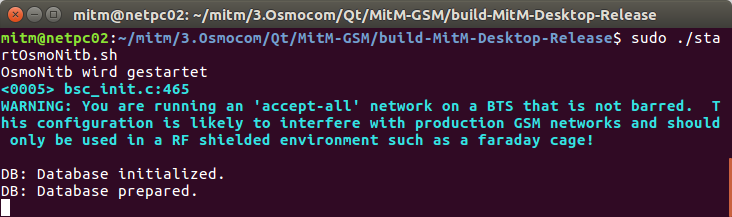
\includegraphics[width=15cm]{includes/Start_OsmoNitb}
\caption{Ansicht der Konsole nach dem Start der OsmoNitb}
\label{fig:OsmoNitb}
\end{figure}

\newpage
OsmoBTS wurde wie folgt gestartet.

\begin{lstlisting}
cd /home/netpc06/osmo-bts/src/osmo-bts-trx
sudo osmo-bts-trx -c osmo-bts.cfg
\end{lstlisting}

\begin{figure}[h] %t=top b=bottom h=here p =eigene page
\centering
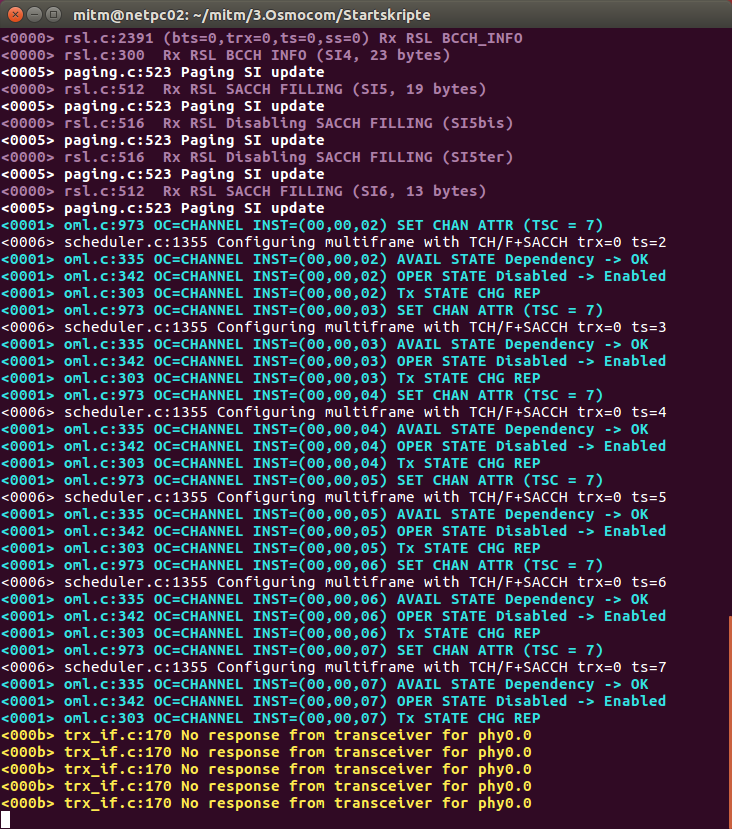
\includegraphics[width=15cm]{includes/Start_OsmoBTS}
\caption{Ansicht der Konsole nach dem Start der OsmoBTS}
\label{fig:OsmoBTS}
\end{figure}


\subsection{Installation weiterer Komponenten}
Neben den Komponenten zur Inbetrienahme des GSM Netzes wurden außerdem weitere Installationen vorgenommen. Diese waren zur Umsetzung des Projektziels notwendig.

\subsubsection{Osmo-sip-Connector}
Zur Konvertierung von .wav-Dateien werden sowohl RTP als auch SIP Pakete benötigt. Um neben RTP und UDP Paketen auch SIP Pakete abfangen zu können, wurde der Osmo-sip-Connector wie folgt installiert.

\begin{lstlisting}
git clone git://git.osmocom.org/osmo-sip-connector.git
cd osmo-sip-connector/
autoreconf -fi
./configure
make
sudo make install
\end{lstlisting} 

Nach erfolgreicher Installation des Osmo-sip-connectors wurde mit Angabe der Konfigurationsdatei gestartet.

\begin{lstlisting}
osmo-sip-connector -c ./osmo-sip-connector.cfg
\end{lstlisting} 

\begin{figure}[h] %t=top b=bottom h=here p =eigene page
\centering
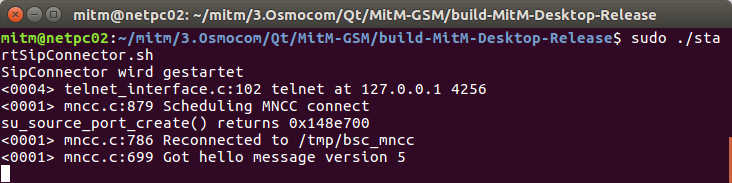
\includegraphics[width=15cm]{includes/Start_SipConnector}
\caption{Ansicht der Konsole nach dem Start des Osmo-sip-connectors}
\label{fig:Asterisk}
\end{figure}
 
\subsubsection{Asterisk}
Den Aufbau von Gesprächen sowie deren Vermittlung wurde in dieser Arbeit der PBX Asterisk verwendet. Dieser wurde über den Paketmanager installiert. Die Einrichtung erforderte die Installation der Bibliothek libsofia-sip-ua-glib-dev.

\begin{lstlisting}
sudo apt-get install asterisk
\end{lstlisting}

Nach der Installation startet Asterisk selbständig. Da mehrmals Änderungen an den Konfigurationsdateien von Asterisk vorgenommen wurden, wurde Asterisk mehrmals neu gestartet.

\begin{lstlisting}
core restart gracefully
sudo asterisk -r
\end{lstlisting}

Nach mehreren Fehlschlägen bezüglich der Installation von Asterisk und folglicher Neuaufsetzen des gesamten Systems inklusive des Betriebssystems wurde Asterisk als erste Komponente vor der GSM Installation eingerichtet. Es stellte sich heraus, dass dieses Vorgehen zu einer erfolgreichen Installation von Asterisk und Inbetriebnahme des GSM Netzes führte.

\begin{figure}[h] %t=top b=bottom h=here p =eigene page
\centering
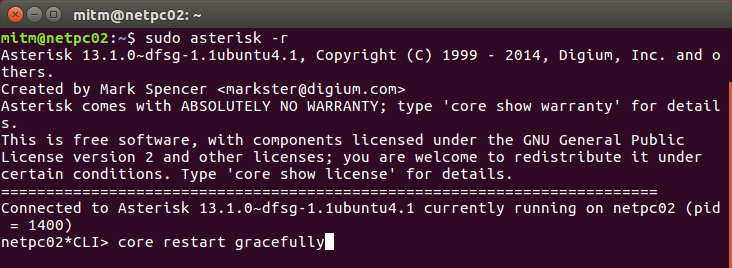
\includegraphics[width=15cm]{includes/Asterisk}
\caption{Ansicht der Konsole nach Verbindung mit Asterisk}
\label{fig:Asterisk}
\end{figure}
\newpage

\section{Inbetriebnahme eines OpenBTS Systems}
Für Inbetriebnahme des GSM Netzes waren einige Vorinstallationen sowie das Einrichten von Ubuntu 16.04.3 nötig. Im Folgenden wird das Vorgehen zur Einrichtung des Systems sowie die Inbetriebnahme des GSM Netzes beschrieben.

\subsection{Vorinstallationen}

\subsubsection{Ubuntu 16.04.3}

Verweis machen, wenn wie bei Osmocom

\subsubsection{Git}

Verweis machen, wenn wie bei Osmocom

\subsubsection{Softwarevoraussetzungen}

selbst

\subsection{Installation einzelner GSM Komponenten}\label{GSM_Komp}

selbst 

\subsection{Starten des Systems}

\newpage
\section{Umsetzung des Projektziels}
Während es sich bei den beiden vorherigen Kapiteln um die Inbetriebnahme des GSM-Netzes selbst gehandelt haben, geht es nun um die konkrete Umsetzung des eigentlichen Projektziels "Man-In-The-Middle". Dabei wird versucht die Gesprächsdaten auf der Strecke zwischen BTS, BSC und PBX abzugreifen.

Zuerst versucht zwischen BTS und BSC?!?
-> evtl Screenshot von Daten des ABIS-Interface?!
https://osmocom.org/projects/osmo-sip-conector/wiki/Osmo-sip-connector
http://ftp.osmocom.org/docs/latest/osmonitb-usermanual.pdf -> p.6/7

Abgreifen der Daten zwischen BTS und BSC (ABIS-Interface) schwierig -> Daten weiter analysiert und weitere Angriffspunkte ausmachen.
-> Abgreifen der Daten vor der Telefonanlage (Asterisk (OPEN: IAX; Osmo: PBX)) -> dadurch die Daten im VOIP Format (SIP + RTP), welches via PC relativ gut zu handeln ist.

Zunächst eigenes analysieren der Daten. Suche nach pratkischem Tool im Internet
-> pcapsipdump

Für die Installation und Einrichtung der benötigten Tools wurde ein Bash-Skript erstellt, welches die meisten Schritte automatisch durchführt. Die manuell noch auszuführenden Schritte werden in der Komandozeile ausgegeben.
\lstinputlisting [caption={Install and configure Script}\label{lst:configure.sh},captionpos=t,language=bash]
{../../4.Projektziel-Umsetzung/configureRecord.sh}


\subsection{pcapsipdump}
\subsection{Abspeichern der Daten}
Mit den beiden Komandozeilenanwendungen tshark und tcpdump können Daten von einem Interface in eine pcap-Datei abgespeichert werden. Hierbei können auch bereits schon beim aufnehmen Filter gesetzt werden, sodass nur die relevanten Daten gespeichert werden.


pcapsipdump ist open-source Tool, welches auf der libpcap basiert. Das Tool hört auf einem Interface die Daten mit und speichert die SIP/RTP sessions als pcap-Datei ab. Diese Datei kann nun in tcpdump, Wireshark oder ähnlichem geöffnet, eingelesen und weiterverarbeitet werden. Das nette Feature dabei ist, dass das Tool selbstständig pro Session eine Datei anlegt. Das Tool läuft als Hintergrundprozess, sodass es nur einmal manuell gestartet werden muss. Alternativ kann das Tool auch mit dem systemd-Init-Prozess automatisch gestartet werden, sofern man es nachträglich selbst konfiguriert.
Hören das Loopback-Interface ab -> da all Tools auf dem selben Rechner laufen und die Tools über diese Schnittstelle miteinander kommunizieren.

Abhängigkeiten des Programms installieren
\begin{lstlisting}
sudo apt-get install -y libpcap-dev
\end{lstlisting}

Gestartet wird das Tool mit folgenden Parametern. 
\begin{lstlisting}
sudo pcapsipdump -i lo -v 10 -d $HOMEPATH/wiresharkCalls/%Y%m%d-%H%M%S-%f-%t-%i.pcap -U
\end{lstlisting}


Im späteren Verlauf Probleme mit dem Tool, sodass letztendlich Source-Code angepasst wurde. Das Problem lag darin, dass das Tool die erstellte Datei lange nicht schließt, obwohl bereits seit längerem die Session beendet ist. Der Übeltäter war ein Timer in der calltable-Klasse, welcher auf 5 Minute gestellt war. Nach Verändern des Timers auf 5 Sekunden wurde auch die erstellte pcap-Datei kurz nach Ende der Session geschlossen.

\begin{lstlisting}[xleftmargin=.04\textwidth, firstnumber=211]
  ...
 if (table[idx].is_used && (
 	(currtime - table[idx].last_packet_time > 5) ||
    (currtime - table[idx].first_packet_time > opt_absolute_timeout))){
  ...
\end{lstlisting}

\subsection{pcap2wavgsm}
\subsection{Extrahieren der Daten}
Zunächst wurden die von pcapsipdump extrahierten Daten mit Wireshark manuell analysiert. Darin sind nun wirklich nur noch die SIP- und RTP-Packet enthalten, wie auf fig XXXXX zu sehen. Mit Wireshark erkennt auch den VOIP-Anruf und kombiniert die RTP-Packages korrekt. Allerdings konnte der Stream nicht direkt im Programm abgespielt werden. Der Grund hierfür ist vermutlich, dass Wireshark gsm nicht dekodieren kann.
Jedoch gibt es einen Weg, wie die beiden Streams als .raw-Daten exportiert werden können. Hierfür ein beliebiges RTP-Packet auswählen, über "Telefonie->RTP->Stream Analyse" den Stream analysieren. Nun kann der Hinweg und Rückweg als seperate Datei gespeichert werden. Man muss jedoch als Datei-Typ .raw auswählen.

Die .raw-Dateien können nun via folgendem Komandozeilenaufruf abgespielt werden
\begin{lstlisting}
padsp play -t gsm -r 8000 -c 1 example.gsm
\end{lstlisting}

Mit dem universellen und sehr mächtigen Audiokonverter SoX können die Dateien über folgenden Komandozeilenaufruf in .wav convertiert werden, sodass diese auch mit jedem herkömmlichen Media Player abgespielt werden können.
\begin{lstlisting}
sox -t gsm -r 8000 -c 1 example.raw exampleConverted.wav
\end{lstlisting}

Mit dem Bash-Skript pcap2wav von https://gist.github.com/avimar/d2e9d05e082ce273962d742eb9acac16 können genau diese Schritte automatisiert ausgeführt werden.


\subsection{Vollautomatisieren aller Schritte}
\subsection{incron}

Das Abspeichern der Daten funktioniert bereits voll automatisiert und jeweils auch in eine extra Datei pro Session. Allerdings muss das Convertierungs-Skript noch automatisch getriggert bzw. ausgeführt werden. Hierfür kann das Linux-Tool "Incron" genutzt werden. Das Tool setzt auf das Kernel-Subsystem Inotify, um auf Dateisystem-Ereignisse zu reagieren. Dadurch kann ein Ordner überwacht werden und bei einer neuen Datei etwas getriggert werden, wie z.B. eben die Ausführung des Konvertierungs-Skriptes. Incron ähnelt dabei in der Handhabung an das Standardwerkzeug "Cron", welches Cron Jobs auf Basis von Zeitpunkten startet.

\begin{lstlisting}
echo ">>installing incron if not already installed.."
if ! which "incrond" > /dev/null
then
	sudo apt-get install -y incron
fi
echo ""
echo ""

echo ">>YOU have to do that manually:"
echo ">>append your username into '/etc/incron.allow'"

echo ">>starting service with 'systemctl start incron.service'"

echo ">>add job with 'incrontab -e' and append following line:"
echo "/home/all/wiresharkCalls IN_CLOSE_WRITE /home/all/startPcap2wavgsmConversion.sh \$@ \$#"
echo ""
\end{lstlisting}

Nun werden also die Daten direkt von der Schnittstelle abgegriffen, gefiltert und gespeichert. Danach automatisch in .wav konvertiert, sodass die Gespräche lokal auf dem PC angehört werden können. Um nicht an den lokalen PC gebunden zu sein, wäre es möglich die Dateien über einen Webserver global zur Verfügung zu stellen.


\subsection{Weiteres Feature}
Es soll das letzte oder die letzten Gespräche via einem Telefonanruf wiedergegeben werden können. Dies wurde mit einer/mehreren speziell konfigurierten Nummern ermöglicht.

==> kann auch die Nummer beschränkt werden, sodass nur eine registrierte Nummer die Gespräche abhören kann?!???
\newpage
\section{Ergebnisse} 
Insgesamt lässt sich sagen, dass die definierten Projektziele in vollem Umfang erreicht wurden. Die Inbetriebnahme des GSM Netzes wurde erfolgreich umgesetzt. Dabei wurden zwei unterschiedliche Architekturen parallel verfolgt, sodass letztendlich zwei verschiedene Netze in Betrieb genommen werden konnten. Aufgrund der geringen Einarbeitungszeit und der begrenzten Projektdauer konnte auf diese Weise sichergestellt werden, dass ein funktionierendes System zur weiteren Verfolgung des Projektzieles zur Verfügung stand. Des Weiteren wurde die Funktionalität des Abgreifens und Abspeicherns eines Telefongesprächs vollständig realisiert. Dabei werden die SIP/RTP Sessions durch das Tool pcapsipdump aufgezeichnet und im .pcap Format gespeichert. Anschließend wird die .pcap Datei in eine .gsm Datei und in das einfacher abspielbare .wav Format konvertiert. Dieses Vorgehen wurde schließlich automatisiert, sodass nach einem getätigten Anruf im Testnetz eine Aufnahme des Gesprächs lokal auf dem Rechner abgespielt werden kann.\\

Außerdem wurde im Projektziel ein optionales Feature formuliert, das ebenfalls vollständig umgesetzt werden konnte. Dieses umfasst die Hinterlegung einer bzw mehreren Rufnummern und das Abspielen des aufgezeichneten Telefongespräches bei Anruf dieser Nummern. Es wurde pro Telefonnummer ein Slot erstellt, sodass immer die letzten Gespräche aller registrierten Teilnehmer abgehört werden können. Zusätzlich wurde nur eine festgelegte IMSI authentifiziert die Gespräche wieder abzuhören, sodass nicht jeder, wer jetzt die Nummern anruft, einfach die Gespräche abhören kann.\\

Beim Vergleich der beiden Architekturen lässt sich sagen, dass bei beiden zunächst einiges installiert und konfiguriert werden musste. Bei Osmocom gab es häufiger das Phänomen, dass beim Beenden eines Anrufs es länger dauerte bis der Anruf dann auch wirklich beendet wurde, sodass die Reaktionszeit bei OpenBTS geringer war. Zudem war die Sprachqualität ebenfalls bei OpenBTS besser bzw klarer. Jedoch ist Osmocom mit den vielen einzelnen Bausteinen, welche auch der realen Welt entsprechen, flexibler, da bei OpenBTS vieles in dem Hauptmodul ist.
Allerdings gibt es keinen klaren Gewinner oder Verlierer.

\section{Fazit}
Durch die effektive Zusammenarbeit sowie team-interne Aufgabenverteilung ergab sich ein rasches Vorankommen. Nichtsdestotrotz ergaben sich Probleme bei der Installation einzelner GSM Komponenten. Das Installieren und Konfigurieren zusätzlicher Abhängigkeiten erschwerte die Inbetriebnahme. So war anfänglich unklar, wie die Konfigurationsdateien von OpenBSC und OsmoBTS auf unsere Anforderungen angepasst werden mussten. Hinzu kamen Probleme beim Kompilieren dieser Dateien. Zur Umsetzung des Projektziels mussten zunächst Recherchen angestellt werden. Da die Vorgehensweise nicht immer eindeutig war, wurden zusätzliche Aufwände für das Ausprobieren mehrerer Möglichkeiten aufgebracht. Alles in allem wurde das Projektziel für alle Beteiligten zur vollkommenen Zufriedenheit zeitgerecht umgesetzt.



\newpage
\section{Projektaufteilung}
Die Aufgaben zur Erreichung des Projektzieles wurden wie folgt verteilt:

\begin{itemize}
\item Inbetriebnahme des GSM Netzes (Attenberger, Bollenmiller, Schuster, Wilhelm)
\item Realisierung der automatisierten Aufzeichnung und Abspeicherung eines Telefonats (Attenberger, Bollenmiller, Schuster, Wilhelm)
\item Hinterlegung einer Rufnummer zur Anhörung des abgespeicherten Telefonats (Attenberger, Bollenmiller, Schuster, Wilhelm)
\item Ausarbeitung und Dokumentation (Attenberger, Bollenmiller, Schuster, Wilhelm)
\end{itemize}

Das Projekt Man-In-The-Middle wurde präsentiert von der J3A Group. \textsuperscript{\textcopyright} J3A MITM

\newpage

\appendix
\chapter{Appendix}
\section{openbsc.cfg} \label{Openbsc.cfg}
\begin{lstlisting}
!
! OpenBSC configuration saved from vty
!   !
password foo
!
line vty
 no login
!
e1\_input
 e1\_line 0 driver ipa
 e1\_line 0 port 0
network
 network country code 262
 mobile network code 99
 short name mitm2
 long name mitm2
 auth policy accept-all
 location updating reject cause 13
 encryption a5 0
 neci 1
 paging any use tch 0
 rrlp mode ms-based
 mm info 1
 handover 0
 handover window rxlev averaging 10
 handover window rxqual averaging 1
 handover window rxlev neighbor averaging 10
 handover power budget interval 6
 handover power budget hysteresis 3
 handover maximum distance 9999
 timer t3101 10
 timer t3113 60
 timer t3122 10
 dtx-used 0
 subscriber-keep-in-ram 0
 bts 0
  type sysmobts
  band PCS1900
  cell\_identity 0
  location\_area\_code 1
  training\_sequence\_code 7
  base\_station\_id\_code 63
  ms max power 0
  cell reselection hysteresis 4
  rxlev access min 0
  periodic location update 30
  channel allocator descending
  rach tx integer 9
  rach max transmission 7
  channel-descrption attach 1
  channel-descrption bs-pa-mfrms 5
  channel-descrption bs-ag-blks-res 1
  ip.access unit\_id 1901 0
  oml ip.access stream\_id 255 line 0
  neighbor-list mode automatic
  trx 0
   rf\_locked 0
   arfcn 806
   nominal power 0
   max\_power\_red 0
   rsl e1 tei 0
    timeslot 0
     phys\_chan\_config CCCH+SDCCH4
     hopping enabled 0
    timeslot 1
     phys\_chan\_config TCH/F
     hopping enabled 0
    timeslot 2
     phys\_chan\_config TCH/F
     hopping enabled 0
    timeslot 3
     phys\_chan\_config TCH/F
     hopping enabled 0
    timeslot 4
     phys\_chan\_config TCH/F
     hopping enabled 0
    timeslot 5
     phys\_chan\_config TCH/F
     hopping enabled 0
    timeslot 6
     phys\_chan\_config TCH/F
     hopping enabled 0
    timeslot 7
     phys\_chan\_config TCH/F
     hopping enabled 0
\end{lstlisting}

\newpage
\section{osmo-bts.cfg}\label{Osmo-bts.cfg}
\begin{lstlisting}
!
! OsmoBTS () configuration saved from vty
!!
!
log stderr
  logging color 1
  logging timestamp 0
  logging level rsl info
  logging level oml info
  logging level rll notice
  logging level rr notice
  logging level meas notice
  logging level pag info
  logging level l1c info
  logging level l1p info
  logging level dsp info
  logging level abis notice
!
line vty
 no login
!
phy 0
 instance 0
 osmotrx rx-gain 1
 osmotrx ip local 127.0.0.1
 osmotrx ip remote 127.0.0.1
bts 0
 band PCS1900
 ipa unit-id 1901 0
 oml remote-ip 127.0.0.1
 paging lifetime 0
 gsmtap-sapi bcch
 gsmtap-sapi ccch
 gsmtap-sapi rach
 gsmtap-sapi agch
 gsmtap-sapi pch
 gsmtap-sapi sdcch
 gsmtap-sapi pacch
 gsmtap-sapi pdtch
 gsmtap-sapi sacch
 trx 0
  phy 0 instance 0
\end{lstlisting}

\newpage
\section{Installations- und Konfigurations-Skript} \label{configureScript}
\lstinputlisting{../../4.Projektziel-Umsetzung/configureRecord.sh}







\section{Quellcode der GUI-Anwendung}

\textbf{Inhalt von main.cpp}

\begin{lstlisting}
#include "mitm.h"
#include <QApplication>

int main(int argc, char *argv[])
{
    QApplication a(argc, argv);
    MitM w;
    w.show();

    return a.exec();
}
\end{lstlisting}



\vspace{2cm}
\textbf{Inhalt von mitm.h}



\begin{lstlisting}
#ifndef MITM_H
#define MITM_H

#include <QMainWindow>
#include <QProcess>

namespace Ui {
class MitM;
}

class MitM : public QMainWindow
{
    Q_OBJECT

public:
    explicit MitM(QWidget *parent = 0);
    ~MitM();

private:
    Ui::MitM *ui;
    QString password;

public slots:
    void checkInput();
    void transceiverPressed();
    void btsPressed();
    void bscPressed();
    void wiresharkPressed();
    void sipConnectorPressed();
    void sqlBrowserPressed();
    void pcapSipDumpPressed();
    void slot1Pressed();
    void slot2Pressed();
    void slot3Pressed();
    void slot4Pressed();
    void slot5Pressed();
};
#endif // MITM_H
\end{lstlisting}



\vspace{2cm}
\textbf{Inhalt von mitm.cpp}

\begin{lstlisting}
#include "mitm.h"
#include "ui_mitm.h"

MitM::MitM(QWidget *parent) :
    QMainWindow(parent),
    ui(new Ui::MitM)
{
    ui->setupUi(this);

    connect(ui->lineEdit, SIGNAL(textEdited(QString)), this, SLOT(checkInput()));
    connect(ui->pushButtonTransceiver, SIGNAL(clicked()), this, SLOT(transceiverPressed()));
    connect(ui->pushButtonBSC, SIGNAL(clicked()), this, SLOT(bscPressed()));
    connect(ui->pushButtonBTS, SIGNAL(clicked()), this, SLOT(btsPressed()));
    connect(ui->pushButtonSipConnector, SIGNAL(clicked()), this, SLOT(sipConnectorPressed()));
    connect(ui->pushButtonWireshark, SIGNAL(clicked()), this, SLOT(wiresharkPressed()));
    connect(ui->pushButtonSQLBrowser, SIGNAL(clicked()), this, SLOT(sqlBrowserPressed()));
    connect(ui->pushButtonPcap, SIGNAL(clicked()), this, SLOT(pcapSipDumpPressed()));
    connect(ui->pushButtonSlot1, SIGNAL(clicked()), this, SLOT(slot1Pressed()));
    connect(ui->pushButtonSlot2, SIGNAL(clicked()), this, SLOT(slot2Pressed()));
    connect(ui->pushButtonSlot3, SIGNAL(clicked()), this, SLOT(slot3Pressed()));
    connect(ui->pushButtonSlot4, SIGNAL(clicked()), this, SLOT(slot4Pressed()));
    connect(ui->pushButtonSlot5, SIGNAL(clicked()), this, SLOT(slot5Pressed()));
}


MitM::~MitM()
{
    delete ui;
}


void MitM::checkInput() {
    password = ui->lineEdit->text();
}


void MitM::transceiverPressed(){

    QProcess* exec = new QProcess(this);

    if (ui->pushButtonTransceiver->isChecked()) {
        exec->start("./startTransceiver.sh");
        ui->pushButtonTransceiver->setText("Stoppen");
    }
    else {
        exec->close();
        ui->pushButtonTransceiver->setText("Starten");
    }
}



void MitM::bscPressed(){

    QProcess* exec = new QProcess(this);

    if (ui->pushButtonBSC->isChecked()) {
        exec->start("./startOsmoNitb.sh");
        ui->pushButtonBSC->setText("Stoppen");
    }
    else {
        exec->close();
        ui->pushButtonBSC->setText("Starten");
    }
}


void MitM::btsPressed(){

    QProcess* exec = new QProcess(this);

    if (ui->pushButtonBTS->isChecked()) {
        exec->start("./startOsmoBTS.sh");
        ui->pushButtonBTS->setText("Stoppen");
    }
    else {
        exec->close();
        ui->pushButtonBTS->setText("Starten");
    }
}



void MitM::wiresharkPressed(){

    QProcess* exec = new QProcess(this);

    if (ui->pushButtonWireshark->isChecked()) {
        exec->start("./wireshark.sh");
        ui->pushButtonWireshark->setText("Stoppen");
    }
    else {
        exec->close();
        ui->pushButtonWireshark->setText("Starten");
    }
}



void MitM::sipConnectorPressed(){

    QProcess* exec = new QProcess(this);

    if (ui->pushButtonSipConnector->isChecked()) {
        exec->start("./startSipConnector.sh");
        ui->pushButtonSipConnector->setText("Stoppen");
    }
    else {
        exec->close();
        ui->pushButtonSipConnector->setText("Starten");
    }
}



void MitM::sqlBrowserPressed(){

    QProcess* exec = new QProcess(this);

    if (ui->pushButtonSQLBrowser->isChecked()) {
        exec->start("./startSQLBrowser.sh");
        ui->pushButtonSQLBrowser->setText("Stoppen");
    }
    else {
        exec->close();
        ui->pushButtonSQLBrowser->setText("Starten");
    }
}



void MitM::pcapSipDumpPressed(){

    QProcess* exec = new QProcess(this);

    if (ui->pushButtonPcap->isChecked()) {
        exec->start("./startPcapSipDump.sh");
        ui->pushButtonPcap->setText("Stoppen");
    }
    else {
        exec->close();
        ui->pushButtonPcap->setText("Starten");
    }
}


void MitM::slot1Pressed(){
    QProcess* exec = new QProcess(this);
    exec->start("./slot1.sh");
}

void MitM::slot2Pressed(){
    QProcess* exec = new QProcess(this);
    exec->start("./slot2.sh");
}

void MitM::slot3Pressed(){
    QProcess* exec = new QProcess(this);
    exec->start("./slot3.sh");
}

void MitM::slot4Pressed(){
    QProcess* exec = new QProcess(this);
    exec->start("./slot4.sh");
}

void MitM::slot5Pressed(){
    QProcess* exec = new QProcess(this);
    exec->start("./slot5.sh");
}
\end{lstlisting}


\vspace{2cm}
\textbf{Inhalt von mitm.ui}

\begin{lstlisting}
<?xml version="1.0" encoding="UTF-8"?>
<ui version="4.0">
 <class>MitM</class>
 <widget class="QMainWindow" name="MitM">
  <property name="geometry">
   <rect>
    <x>0</x>
    <y>0</y>
    <width>648</width>
    <height>330</height>
   </rect>
  </property>
  <property name="windowTitle">
   <string>MitM</string>
  </property>
  <widget class="QWidget" name="centralWidget">
   <widget class="QGroupBox" name="groupBox">
    <property name="geometry">
     <rect>
      <x>10</x>
      <y>10</y>
      <width>341</width>
      <height>311</height>
     </rect>
    </property>
    <property name="title">
     <string>GSM-Netz erzeugen</string>
    </property>
    <widget class="QLabel" name="label">
     <property name="geometry">
      <rect>
       <x>20</x>
       <y>40</y>
       <width>171</width>
       <height>17</height>
      </rect>
     </property>
     <property name="text">
      <string>Administratorpasswort:</string>
     </property>
    </widget>
    <widget class="QPushButton" name="pushButtonWireshark">
     <property name="geometry">
      <rect>
       <x>230</x>
       <y>230</y>
       <width>99</width>
       <height>27</height>
      </rect>
     </property>
     <property name="text">
      <string>Starten</string>
     </property>
     <property name="checkable">
      <bool>true</bool>
     </property>
    </widget>
    <widget class="QLabel" name="label_4">
     <property name="geometry">
      <rect>
       <x>20</x>
       <y>160</y>
       <width>81</width>
       <height>17</height>
      </rect>
     </property>
     <property name="text">
      <string>OsmoBTS:</string>
     </property>
    </widget>
    <widget class="QLabel" name="label_6">
     <property name="geometry">
      <rect>
       <x>20</x>
       <y>240</y>
       <width>91</width>
       <height>17</height>
      </rect>
     </property>
     <property name="text">
      <string>Wireshark:</string>
     </property>
    </widget>
    <widget class="QLabel" name="label_2">
     <property name="geometry">
      <rect>
       <x>20</x>
       <y>80</y>
       <width>111</width>
       <height>17</height>
      </rect>
     </property>
     <property name="text">
      <string>Transceiver:</string>
     </property>
    </widget>
    <widget class="QLabel" name="label_3">
     <property name="geometry">
      <rect>
       <x>20</x>
       <y>120</y>
       <width>91</width>
       <height>17</height>
      </rect>
     </property>
     <property name="text">
      <string>OsmoBSC:</string>
     </property>
    </widget>
    <widget class="QPushButton" name="pushButtonSipConnector">
     <property name="geometry">
      <rect>
       <x>230</x>
       <y>190</y>
       <width>99</width>
       <height>27</height>
      </rect>
     </property>
     <property name="text">
      <string>Starten</string>
     </property>
     <property name="checkable">
      <bool>true</bool>
     </property>
    </widget>
    <widget class="QPushButton" name="pushButtonSQLBrowser">
     <property name="geometry">
      <rect>
       <x>230</x>
       <y>270</y>
       <width>99</width>
       <height>27</height>
      </rect>
     </property>
     <property name="text">
      <string>Starten</string>
     </property>
     <property name="checkable">
      <bool>true</bool>
     </property>
    </widget>
    <widget class="QLineEdit" name="lineEdit">
     <property name="geometry">
      <rect>
       <x>230</x>
       <y>30</y>
       <width>101</width>
       <height>27</height>
      </rect>
     </property>
     <property name="echoMode">
      <enum>QLineEdit::Password</enum>
     </property>
    </widget>
    <widget class="QPushButton" name="pushButtonTransceiver">
     <property name="geometry">
      <rect>
       <x>230</x>
       <y>70</y>
       <width>99</width>
       <height>27</height>
      </rect>
     </property>
     <property name="text">
      <string>Starten</string>
     </property>
     <property name="checkable">
      <bool>true</bool>
     </property>
    </widget>
    <widget class="QLabel" name="label_5">
     <property name="geometry">
      <rect>
       <x>20</x>
       <y>200</y>
       <width>111</width>
       <height>17</height>
      </rect>
     </property>
     <property name="text">
      <string>Sip-Connector:</string>
     </property>
    </widget>
    <widget class="QPushButton" name="pushButtonBTS">
     <property name="geometry">
      <rect>
       <x>230</x>
       <y>150</y>
       <width>99</width>
       <height>27</height>
      </rect>
     </property>
     <property name="text">
      <string>Starten</string>
     </property>
     <property name="checkable">
      <bool>true</bool>
     </property>
    </widget>
    <widget class="QPushButton" name="pushButtonBSC">
     <property name="geometry">
      <rect>
       <x>230</x>
       <y>110</y>
       <width>99</width>
       <height>27</height>
      </rect>
     </property>
     <property name="text">
      <string>Starten</string>
     </property>
     <property name="checkable">
      <bool>true</bool>
     </property>
    </widget>
    <widget class="QLabel" name="label_7">
     <property name="geometry">
      <rect>
       <x>20</x>
       <y>270</y>
       <width>121</width>
       <height>17</height>
      </rect>
     </property>
     <property name="text">
      <string>SQLiteBrowser:</string>
     </property>
    </widget>
   </widget>
   <widget class="QGroupBox" name="groupBox_2">
    <property name="geometry">
     <rect>
      <x>360</x>
      <y>10</y>
      <width>281</width>
      <height>311</height>
     </rect>
    </property>
    <property name="title">
     <string>Gesprach ausspahen</string>
    </property>
    <widget class="QLabel" name="label_8">
     <property name="geometry">
      <rect>
       <x>20</x>
       <y>40</y>
       <width>111</width>
       <height>17</height>
      </rect>
     </property>
     <property name="text">
      <string>PcapSipDump:</string>
     </property>
    </widget>
    <widget class="QPushButton" name="pushButtonPcap">
     <property name="geometry">
      <rect>
       <x>170</x>
       <y>40</y>
       <width>89</width>
       <height>25</height>
      </rect>
     </property>
     <property name="text">
      <string>Starten</string>
     </property>
     <property name="checkable">
      <bool>true</bool>
     </property>
    </widget>
    <widget class="QPushButton" name="pushButtonSlot1">
     <property name="geometry">
      <rect>
       <x>170</x>
       <y>110</y>
       <width>89</width>
       <height>25</height>
      </rect>
     </property>
     <property name="text">
      <string>Slot 1</string>
     </property>
    </widget>
    <widget class="QPushButton" name="pushButtonSlot2">
     <property name="geometry">
      <rect>
       <x>170</x>
       <y>150</y>
       <width>89</width>
       <height>25</height>
      </rect>
     </property>
     <property name="text">
      <string>Slot 2</string>
     </property>
    </widget>
    <widget class="QPushButton" name="pushButtonSlot3">
     <property name="geometry">
      <rect>
       <x>170</x>
       <y>190</y>
       <width>89</width>
       <height>25</height>
      </rect>
     </property>
     <property name="text">
      <string>Slot 3</string>
     </property>
    </widget>
    <widget class="QPushButton" name="pushButtonSlot4">
     <property name="geometry">
      <rect>
       <x>170</x>
       <y>230</y>
       <width>89</width>
       <height>25</height>
      </rect>
     </property>
     <property name="text">
      <string>Slot 4</string>
     </property>
    </widget>
    <widget class="QPushButton" name="pushButtonSlot5">
     <property name="geometry">
      <rect>
       <x>170</x>
       <y>270</y>
       <width>89</width>
       <height>25</height>
      </rect>
     </property>
     <property name="text">
      <string>Slot 5</string>
     </property>
    </widget>
   </widget>
  </widget>
 </widget>
 <layoutdefault spacing="6" margin="11"/>
 <resources/>
 <connections/>
</ui>
\end{lstlisting}




%%HIER ENDET DIE ARBEIT! DER REST IST KOMMENTAR MIT EIN PAAR PRAKTISCHEN FORMATIERUNGEN!!
\end{document}



%%%%%EINIGE SEHR PRAKTISCHE FORMATIERUNGSBEFEHLE UM ALLES SCHÖN UND EINHEITLICH AUSSEHEN ZU LASSEN!!%%%%%%%
%%%%%%%%%%%%%%%%%%%%%%%%%%%%%%%%%%%%%%%%%%%%%%%%%%%%%%%%%%%%%%%%%%%%%%%%%%%%%%%%%%%%%%%%%%%%%%%%%%%%%%%%%%%
%%%%%%%%%%%%%%%%%%%%%COMMENT%%%%%%%%%%%%%%%%%%%%%%COMMENT%%%%%%%%%%%%%%%%%%%%%%COMMENT%%%%%%%%%%%%%%%%%%%%%
%%%%%%%%%%%%%%%%%%%%%%%%%%%%%%%%%%%%%%%%%%%%%%%%%%%%%%%%%%%%%%%%%%%%%%%%%%%%%%%%%%%%%%%%%%%%%%%%%%%%%%%%%%%
\begin{comment}

% FORMELN UND PARAMETERBESCHREIBUNGEN
\begin{align}
\Delta \varphi = 360^\circ \cdot \frac{\Delta t}{T} = 360^\circ \cdot \Delta t \cdot f
\end{align}
wobei:
\begin{conditions} % *sternchen für zeilenübergreifende beschreibungstexte!!!
\Delta \varphi	& Phasenverschiebung \\
\Delta t		& Zeitdifferenz zwischen Eingangsspannung und gedämpfter Ausgangsspannung\\
T				& Periodendauer der Eingangsspannung \\
f				& Frequenz der Eingangsspannung
\end{conditions}

% Aufrechte griechische Buchstaben für Einheiten
\upmu
\upalpha
...etc

% BILDER EINFÜGEN
\begin{figure}[h] %t=top b=bottom h=here p =eigene page
\centering
\includegraphics[width=15cm]{media/hohlleiter}
\caption{Versuchsaufbau Hohlleiter}
\label{fig:label}
\end{figure}

% MEHRERE BILDER NEBENEINANDER
\begin{figure}[h] %t=top b=bottom h=here p =eigene page 
\flushright
\subfloat[Dispersionsrelation]{\includegraphics[width=7cm]{media/dispers}}
\subfloat[Phasen- und Gruppengeschwindigkeit]{\includegraphics[width=7cm]{media/phasgrupp}}
\end{figure}

%BILDER VOM TEXT UMFLOSSEN
\begin{wrapfigure}[10]{r}{8cm}
\centering
\includegraphics[width=7cm]{media/bragg}
\caption{\textsl{Aufbau eines Bragg-Spektrometers}}
\label{fig:bragg}
\end{wrapfigure}

%TABELLEN
\begin{table}[h]
\centering
\begin{tabular}{|c|c|}
\hline
$z$ [mm] & $\Delta z$ [mm]\\
\hline
3,3 & 0 \\
4,9 & 1,6 \\
6,5 & 1,6 \\
8,0 & 1,5 \\
\hline
\end{tabular}
\caption{Position der Minima zueinander und jeweiliger gemessener Abstand}
\label{tab:label}
\end{table}

% VERBUNDENE ZELLEN IN TABELLEN
\begin{table}[h]
\centering
\begin{tabular}{|c|c|c|c|p{1cm}p{1cm}p{1cm}p{1cm}p{1cm}p{1cm}p{1cm}|}
\hline
A & B & C & D & \multicolumn{7}{|c|}{F}  \\ \hline
\multirow{ 2}{*}{1} & 0 & 6 & 230 & 35 & 40 & 55 & 25 & 40 & 35 & \\
& 1 & 5 & 195 & 25 & 50 & 35 & 40 & 45 &  &  \\ \hline
\end{tabular}
\caption{A test caption}
\label{tab:table2}
\end{table}

% MEHRERE TABELLEN NEBENEINANDER
\begin{table}[h]
\centering

\subfloat[PVC, $d=15,0\,$mm]{
\begin{tabular}[b]{|c|c|c|}
\hline
mit Platte & ohne Platte & $\Delta s$\\
\hline
3,6 & 4,85 & 1,25\\
3,55 & 4,8 & 1,25\\
3,5 & 4,75 & 1,25\\
3,55 & 4,85 & 1,3\\
\hline
\end{tabular}
}

\subfloat[PE, $d=12,2\,$mm]{
\begin{tabular}[b]{|c|c|c|}
\hline
mit Platte & ohne Platte & $\Delta s$\\
\hline
3,5 & 4,2 & 0,7\\
3,5 & 4,25 & 0,75\\
3,5 & 4,2 & 0,7\\
\hline
\end{tabular}
}

\caption{Materialproben und zugehörige Messwerte in [cm]}
\end{table}

% FLOATS ERZWINGEN = TABELLEN UND BILDER ZWINGEND EINFÜGEN
\FloatBarrier

% ABSÄTZE MIT EINSTELLBARER UND NACHTRÄGLICH GLOBAL ÄNDERBARER DISTANZ
\mypar

% PDFs ANHÄNGEN
\includepdf[pages=-]{media/protokoll}

%BILDER UND TABELLEN REFERENZIEREN
\ref{labelname}
\pageref{labelname}

%REFERENZIERUNGSREGELN ZUR ÜBERSICHTLICHKEIT
bilder: fig:label
tabellen: tab:label
gleichungen: eq:label

\end{comment}
%%%%%%%%%%%%%%%%%%%%%%%%%%%%%%%%%%%%%%%%%%%%%%%%%%%%%%%%%%%%%%%%%%%%%%%%%%%%%%%%%%%%%%%%%%%%%%%%%%%%%%%%%%%
%%%%%%%%%%%%%%%%%%%%%COMMENT%%%%%%%%%%%%%%%%%%%%%%COMMENT%%%%%%%%%%%%%%%%%%%%%%COMMENT%%%%%%%%%%%%%%%%%%%%%
%%%%%%%%%%%%%%%%%%%%%%%%%%%%%%%%%%%%%%%%%%%%%%%%%%%%%%%%%%%%%%%%%%%%%%%%%%%%%%%%%%%%%%%%%%%%%%%%%%%%%%%%%%%
